\chapter{\acrshort{ui} and Usability}
\label{user_interface_and_usability}

The final \gls{SafeVision} \acrshort{ui} is presented in this Chapter, with emphasis on how it supports the hybrid redaction workflow. The interface was developed to remain consistent with Safe Media AI's existing platform while adapting the workflow to visual media. Further discussion of the UI theory, design principles, and interface evolution is provided in Appendix~\ref{app:depth_ui_ux}.

\section{Interface Design and Components}

As shown in Figure~\ref{fig:ui_final_examples} (a), the interface starts in an intentionally minimal state. Before files are uploaded, users are presented with a clear upload action and an empty file panel. By avoiding unnecessary controls before they become relevant, the design supports simplicity. Once files are uploaded, the interface expands into the full editing workspace shown in Figure~\ref{fig:ui_final_examples} (b).

On the left side, the file panel gives users an overview of uploaded images and videos. Each file item displays basic information such as file name and file type. During longer operations, individual progress indicators can also be shown for each file, as illustrated in Figure~\ref{fig:file_progress}. Providing this feedback improves system state awareness, especially when \gls{SafeVision} processes several files and users need to understand which file is selected, which task is running, and how far the operation has progressed.

\begin{figure}[H]
\centering
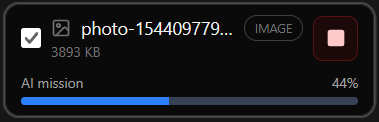
\includegraphics[width=0.55\textwidth]{figures/images/chapter-6/uikomp01.png}
\caption{File item showing individual progress feedback during processing.}
\label{fig:file_progress}
\end{figure}

At the center of the interface, the workspace functions as the main interaction area. Uploaded images and videos are displayed in the middle of the screen so users can inspect the visual content being processed without switching between separate views. By showing detection results directly on the media, the interface reduces the need to compare separate lists or external outputs, which helps lower cognitive load. After identification is completed, detected regions appear as labeled \gls{bounding box}es on the image or video frame, as shown in Figures~\ref{fig:ui_final_examples} (c) and~\ref{fig:video_detection_results}. Using overlays and labeled \gls{bounding box}es reflects the principle of visual feedback \cite{norman2013design}. Detection results appear directly where the sensitive content is located, making the system output easier to understand. As a result, users can assess whether the detected regions are correct, remove \gls{false positive}s, or add missing regions manually.

%----------------
\begin{figure}[H]
    \centering

    \begin{minipage}{\textwidth}
        \centering
        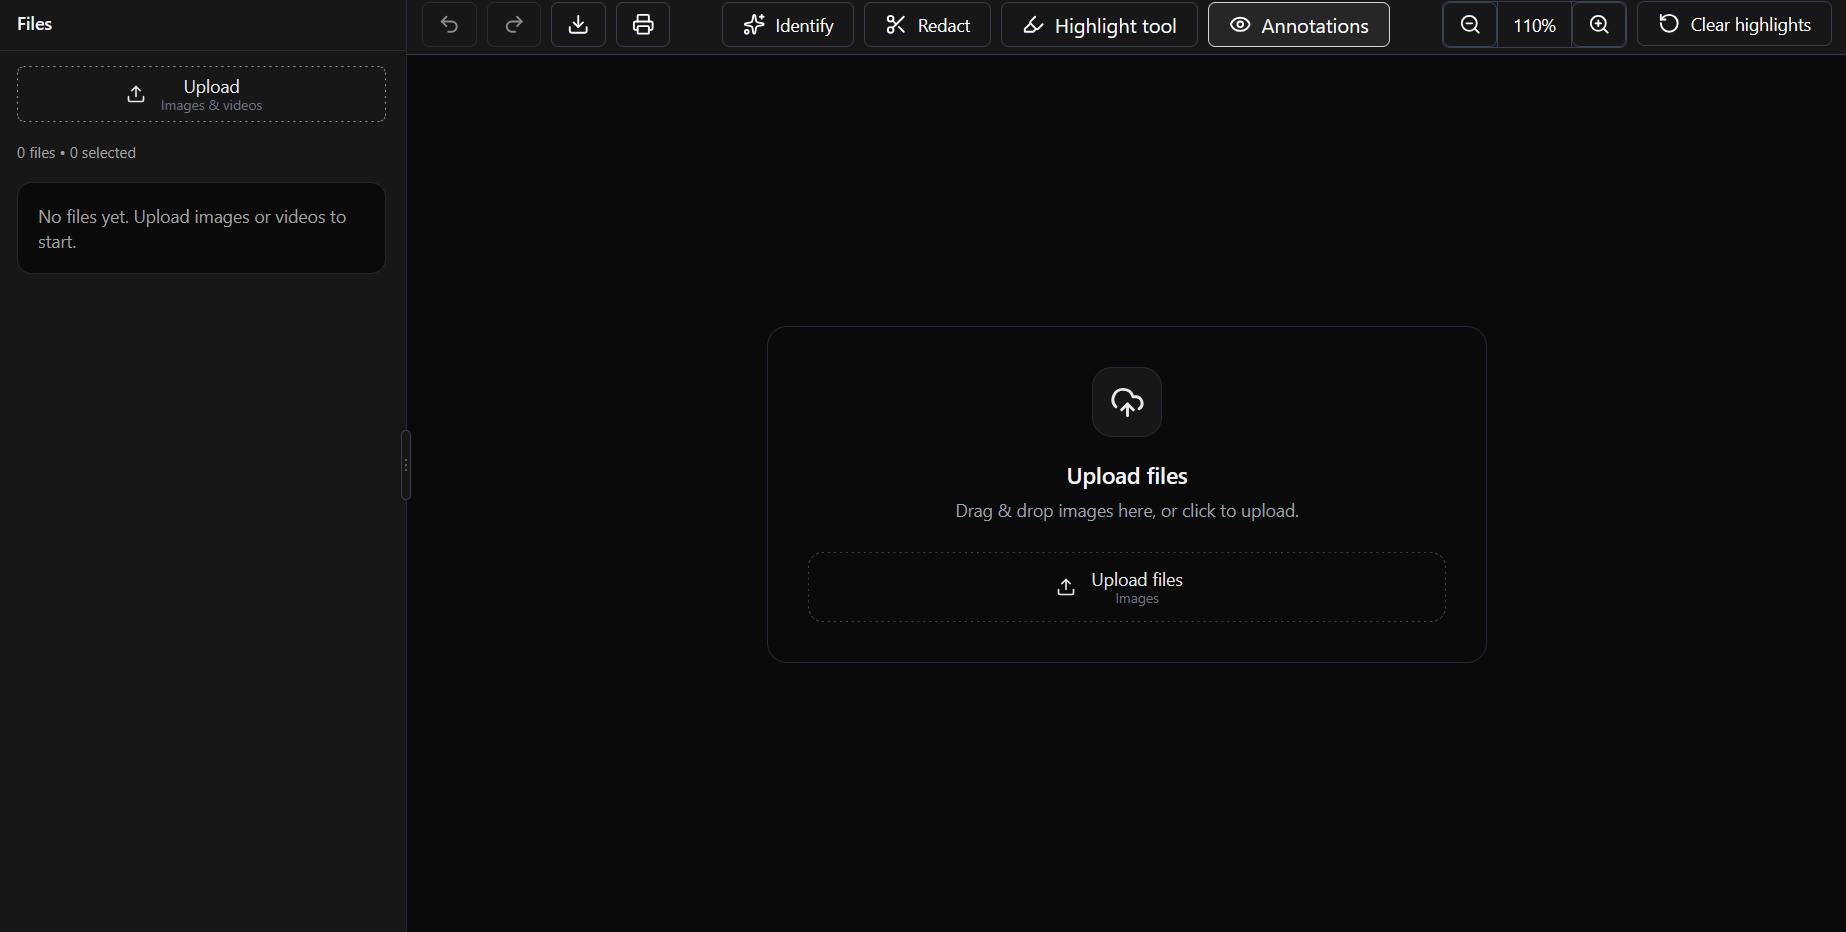
\includegraphics[width=0.7\textwidth]{figures/images/chapter-6/uislutt01.png}
        \par\vspace{2pt} \small (a) Final interface in its initial state before files are uploaded.
    \end{minipage}

    \vspace{0.0cm}

    \begin{minipage}{\textwidth}
        \centering
        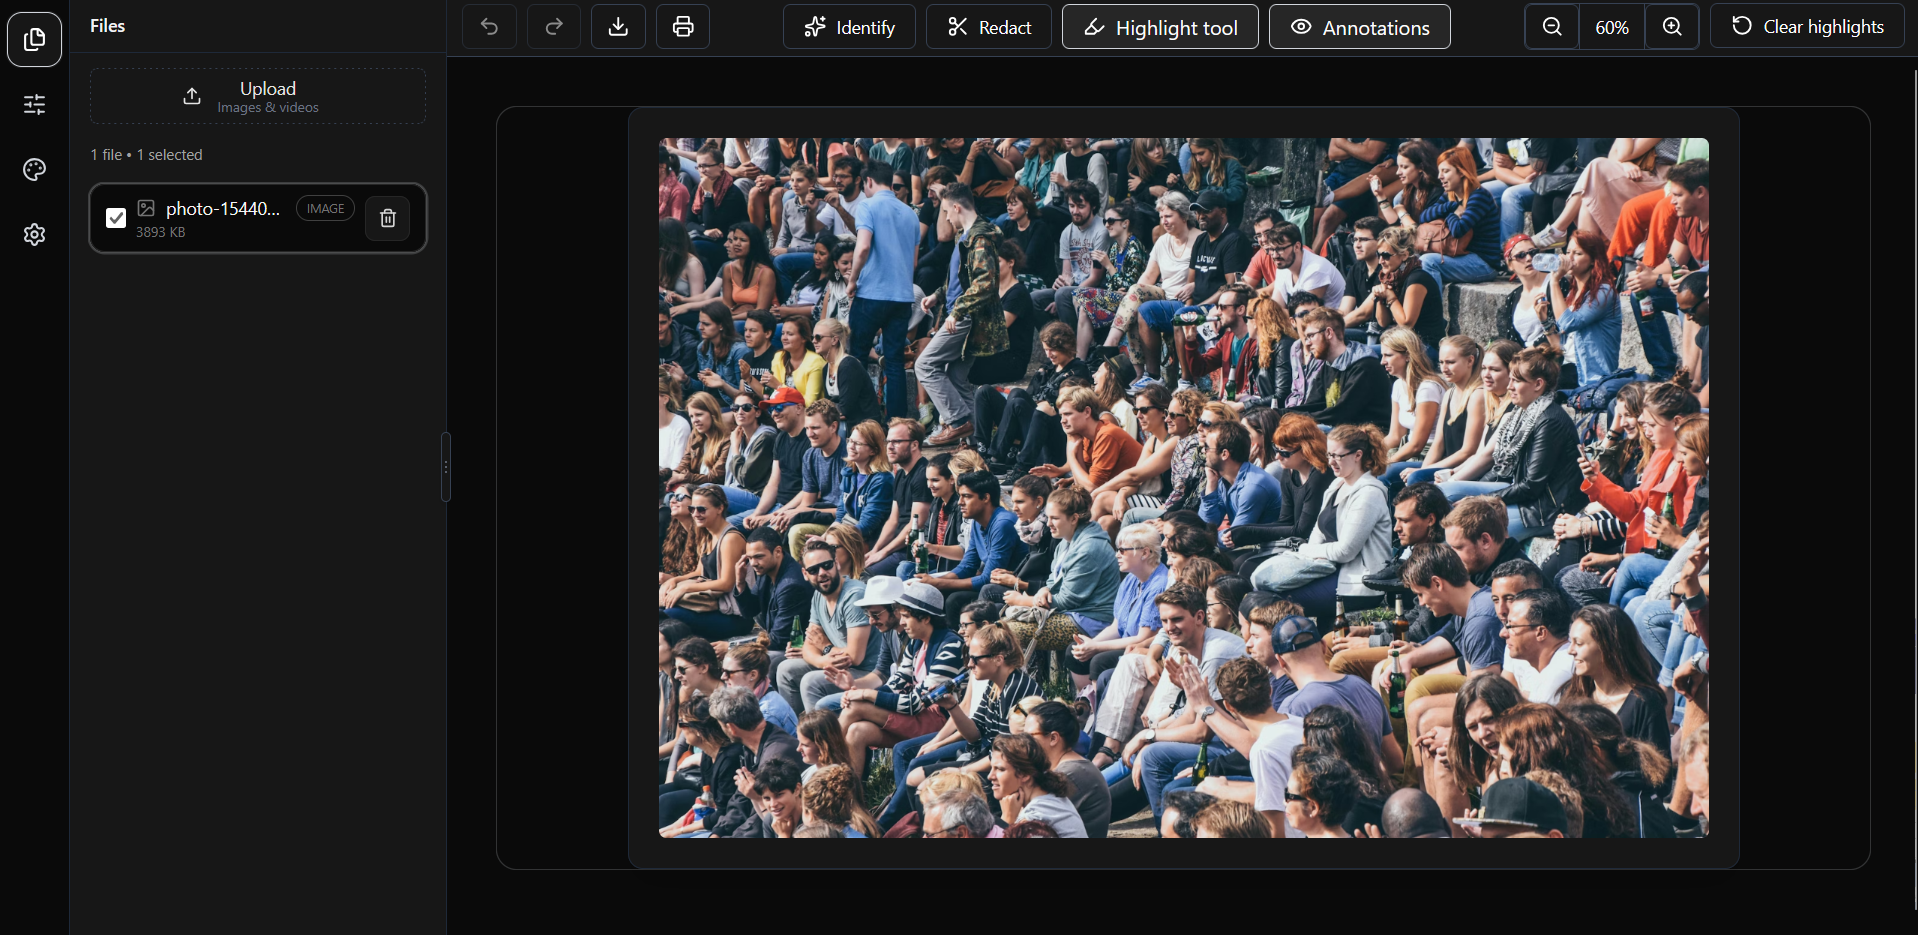
\includegraphics[width=0.7\textwidth]{figures/images/chapter-6/uislutt02.png}
        \par\vspace{2pt} \small (b) Final image workspace with uploaded media displayed in the central viewer.
    \end{minipage}

    \vspace{0.0cm}
    
    \begin{minipage}{\textwidth}
        \centering
        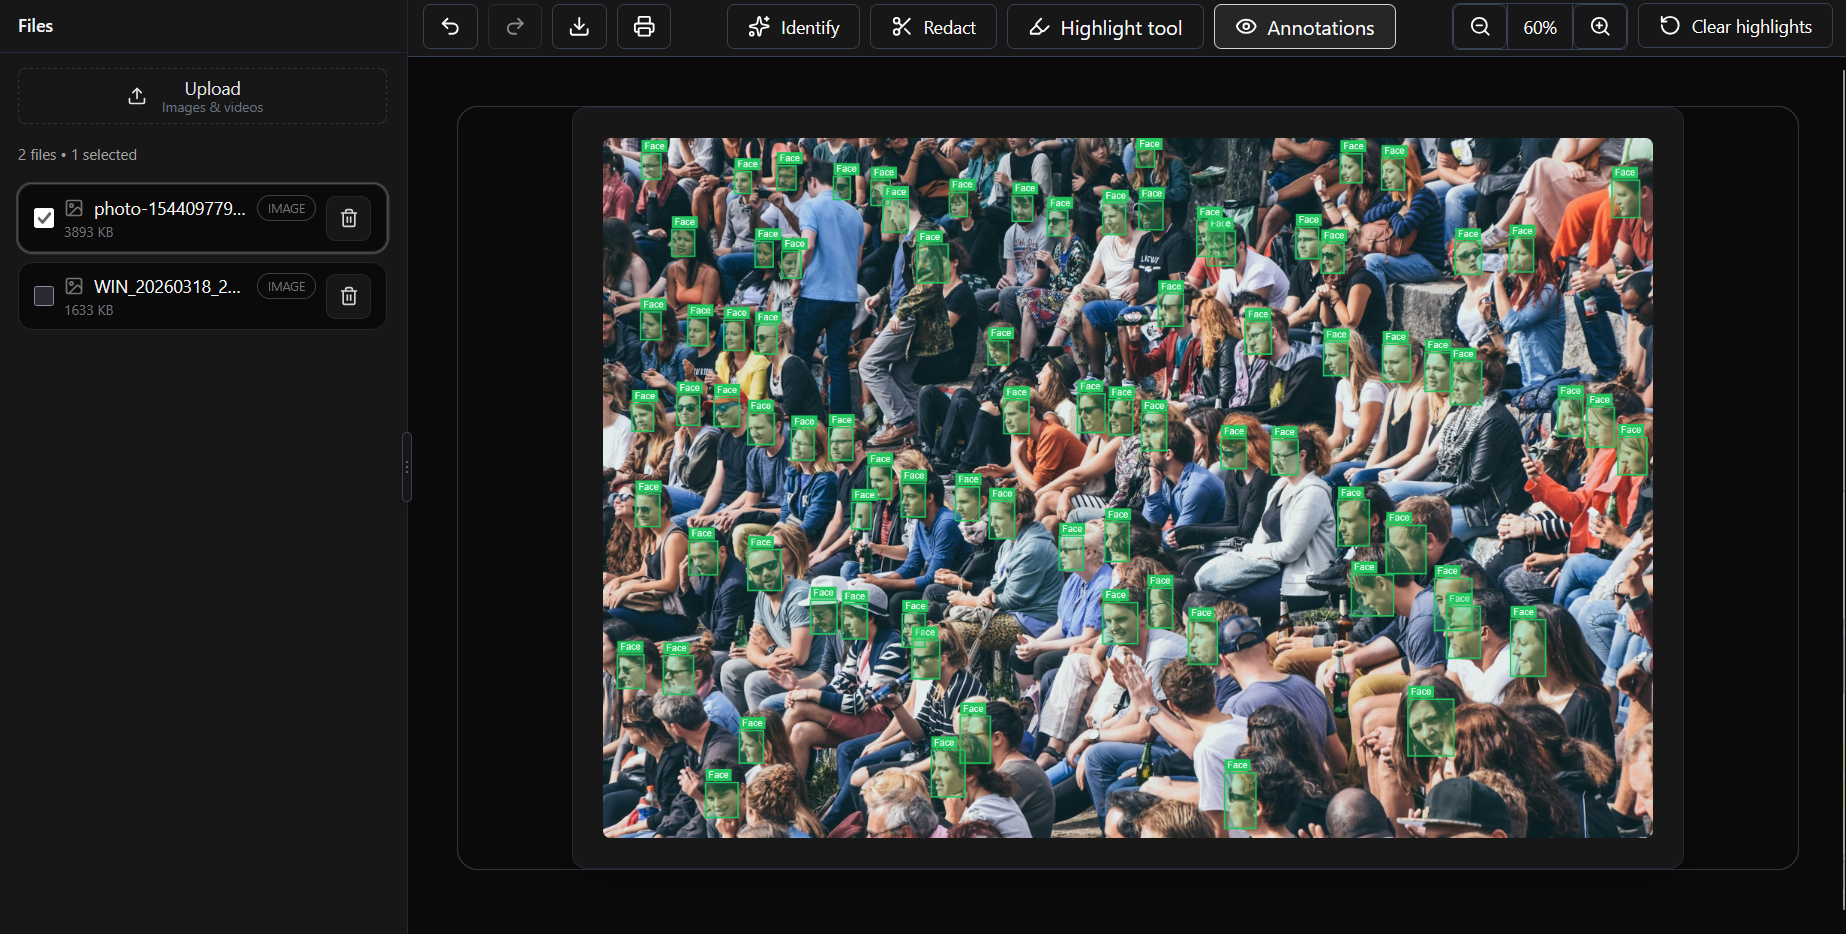
\includegraphics[width=0.7\textwidth]{figures/images/chapter-6/uislutt03.png}
        \par\vspace{2pt} \small (c) Detection results displayed directly on the image using labelled \gls{bounding box}es.
    \end{minipage}

    \caption{Examples of the finalinterface across different stages of the image workflow, from the initial state to uploaded media and displayed detection results. The image used in the workspace examples is from Guillemot~\cite{guillemot_stadium}}
    \label{fig:ui_final_examples}
\end{figure}
%----------------
 
Primary actions are placed in the top toolbar to reflect the intended workflow. By keeping these controls consistently above the workspace as illustrated in Figure~\ref{fig:ui_final_examples}, the main workflow remains visible and predictable throughout the redaction process. 

As shown in Figure~\ref{fig:options_panel_components} (a), secondary and advanced settings are placed in the side panel. Instead of showing every configuration option in the main workspace, settings related to both image and video handling are grouped separately. Advanced functionality therefore remains available without overwhelming the basic workflow, which supports progressive disclosure \cite{nielsen2020progressive}. In practice, this keeps the interface simple for new users while still giving more experienced users additional control when needed. Detection filters allow users to choose which categories should be identified (b). This gives the users flexibility over the hybrid workflow. The same design logic is also applied for video options, Figure~\ref{fig:options_video_rate}. The interface therefore includes components for image visualization, control panels, and editing tools, enabling users to inspect detected regions and apply redaction methods while maintaining clarity and responsiveness, which are central usability principles \cite{usability_nielsen}.

\begin{figure}[H]
\centering

\begin{subfigure}[t]{0.32\textwidth}
    \centering
    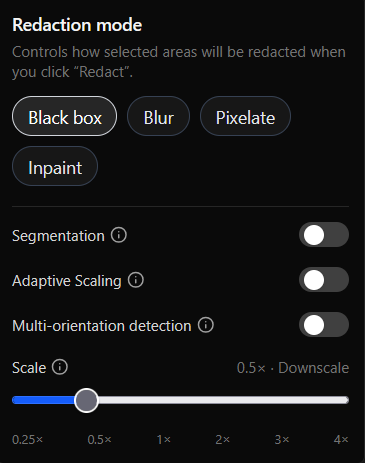
\includegraphics[width=\textwidth]{figures/images/chapter-6/uikomp05.png}
    \caption{Redaction mode and processing settings.}
    \label{fig:options_redaction_mode}
\end{subfigure}
\hfill
\begin{subfigure}[t]{0.32\textwidth}
    \centering
    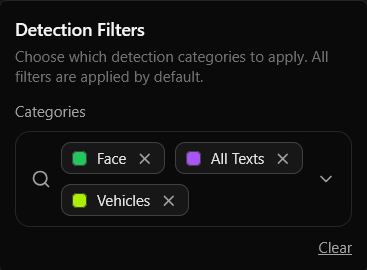
\includegraphics[width=\textwidth]{figures/images/chapter-6/uikomp06.png}
    \caption{Detection filters.}
    \label{fig:options_detection_filters}
\end{subfigure}
\hfill
\begin{subfigure}[t]{0.32\textwidth}
    \centering
    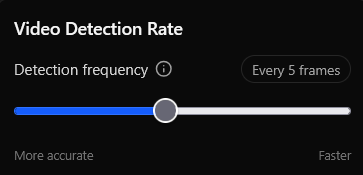
\includegraphics[width=\textwidth]{figures/images/chapter-6/uikomp07.png}
    \caption{Video detection rate.}
    \label{fig:options_video_rate}
\end{subfigure}

\caption{Main components of the options panel. The panel provides access to redaction modes and processing settings, detection filters, and video detection rate configuration.}
\label{fig:options_panel_components}
\end{figure}

Figure~\ref{fig:highlight_styles} (a), the highlight style panel controls how \gls{bounding box}es are displayed. Such customization is important because \gls{SafeVision} may be used on complex images or videos where one default highlight style may not always be readable. Customizable highlighting therefore improves visual feedback and accessibility during detailed inspection tasks.

\begin{figure}[H]
\centering

\begin{subfigure}[t]{0.32\textwidth}
    \centering
    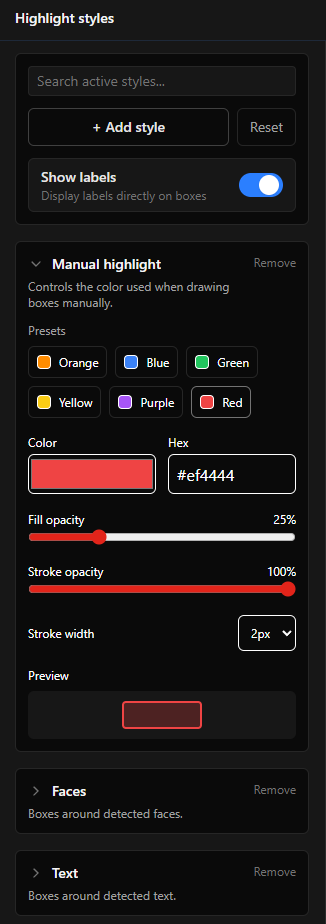
\includegraphics[width=\textwidth]{figures/images/chapter-6/uikomp03.png}
    \caption{Highlight style panel for customizing labels, colors, opacity, and category-specific styles.}
    \label{fig:highlight_styles}
\end{subfigure}
\hfill
\begin{subfigure}[t]{0.32\textwidth}
    \centering
    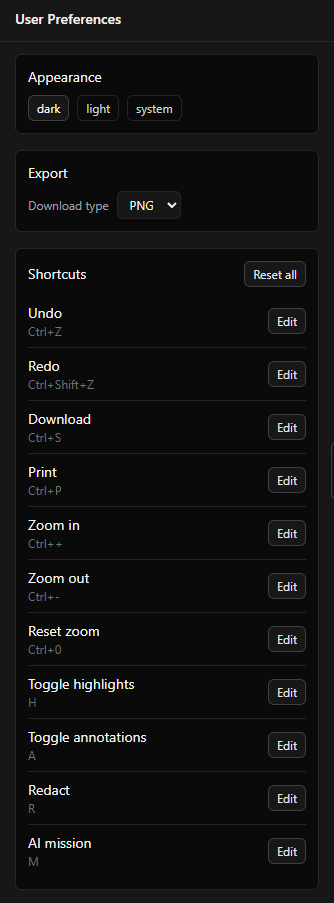
\includegraphics[width=\textwidth]{figures/images/chapter-6/uikomp04.png}
    \caption{User preferences panel with appearance settings, export format, and keyboard shortcuts.}
    \label{fig:user_preferences}
\end{subfigure}

\caption{Configuration panels for highlight styling and user preferences.}
\label{fig:ui_configuration_panels}
\end{figure}

Additional flexibility is provided through the user preferences panel, shown in Figure~\ref{fig:user_preferences}. Users can adapt the interface to different working conditions and make frequent actions faster through personalized settings. At the same time, important functionality remains available through visible interface controls, so the system does not depend on shortcut use. In this way, the preferences panel supports both accessibility and learnability.

Video support extends the same workspace principles to temporal media. As shown in Figure~\ref{fig:video_workspace}, videos are displayed in the central viewer with playback controls, while the surrounding interface remains consistent with the image workflow. After identification, detected regions can be shown on the video frame, as illustrated in Figure~\ref{fig:video_detection_results}. This consistency helps users transfer knowledge from image redaction to video redaction. At the same time, video introduces additional complexity because detections must be interpreted across frames, making clear visual feedback and playback control especially important.

\begin{figure}[H]
\centering

\begin{subfigure}[t]{0.95\textwidth}
    \centering
    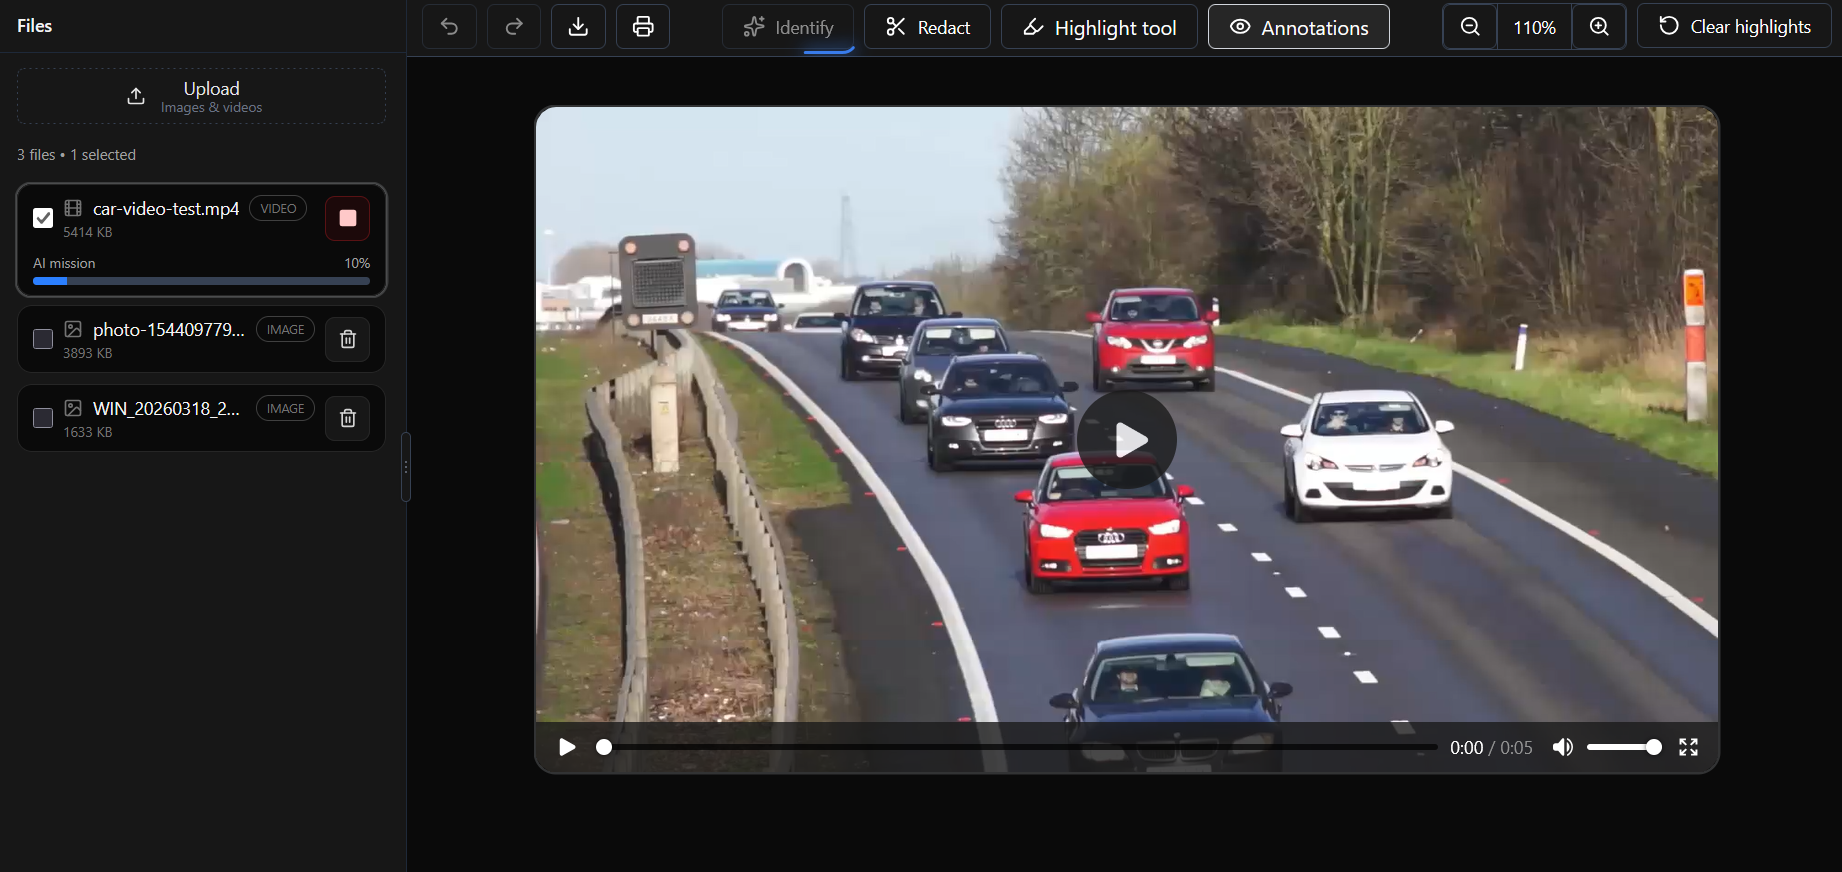
\includegraphics[width=\textwidth]{figures/images/chapter-6/uislutt04.png}
    \caption{Video workspace showing uploaded video content in the central viewer.}
    \label{fig:video_workspace}
\end{subfigure}

\vspace{0.2cm}

\begin{subfigure}[t]{0.95\textwidth}
    \centering
    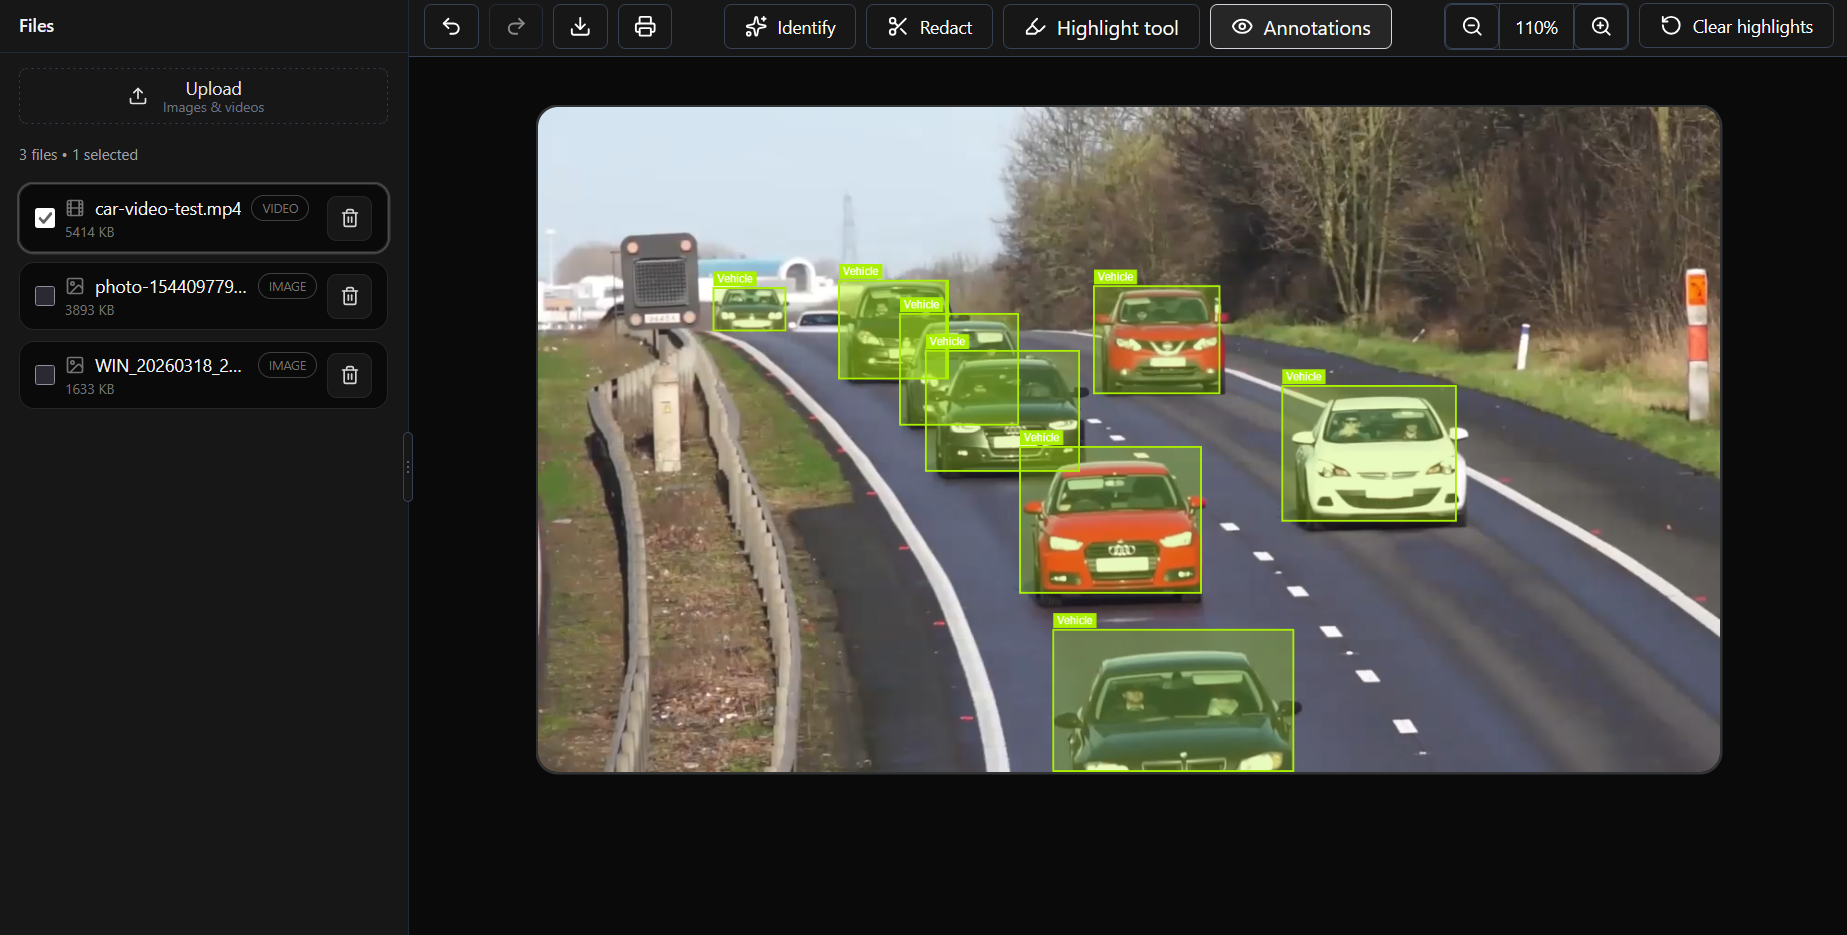
\includegraphics[width=\textwidth]{figures/images/chapter-6/uislutt05.png}
    \caption{Detected vehicle regions displayed on a video frame.}
    \label{fig:video_detection_results}
\end{subfigure}

\caption{Examples of the final \gls{SafeVision} video workflow, showing uploaded video content and detected vehicle regions. The video used in the workspace examples is from ~\cite{pexels_highway_video}.}
\label{fig:video_workflow_examples}
\end{figure}

In the final interface, the design principles described in the previous subsections are applied to the practical needs of \gls{SafeVision}. A single workspace layout keeps the main workflow in one place, while editable detections and configurable settings allow users to stay in control of automated results. Feedback during detection and redaction is provided directly through the interface, and consistent toolbar and panel structures make the workflow more predictable across both image and video processing. Together, these design choices support \gls{SafeVision}'s main goal of combining automated detection with user-guided refinement, so that sensitive visual content can be identified, verified, and redacted in an efficient and controlled workflow.

\section{User Guidance and System Communication}
\label{sec:user_guidance_system_communication}

In addition to the main redaction workflow, the interface includes supporting elements for user guidance and system communication. A short Terms of Service dialog is shown before users begin processing content. This informs users that automated redaction may be inaccurate or incomplete, and that they remain responsible for reviewing results before sharing or publishing processed media. The full Terms of Service text is included in Appendix~\ref{app:terms_of_service}. This was included to make the limitations of automated redaction clearer and to support the responsible use of the system.

The interface also includes a compact patch notes dialog that summarizes important changes between versions, such as performance improvements, image processing changes, video support, and detection updates. This helps communicate system changes to users without requiring them to inspect technical documentation. The patch notes were kept short and limited on user visible changes, since their purpose is to support transparency rather than provide a detailed development log. Examples of these supporting dialog are shown in Figure~\ref{fig:user_guidance_dialogs}.

\begin{figure}[H]
    \centering

    \begin{subfigure}[t]{0.495\textwidth}
        \centering
        \includegraphics[width=\textwidth, trim=35 35 35 35, clip]{figures/images/chapter-6/terms1.png}
        \caption{Terms dialog requiring user confirmation before processing.}
        \label{fig:terms_required}
    \end{subfigure}
    \hfill
    \begin{subfigure}[t]{0.495\textwidth}
        \centering
        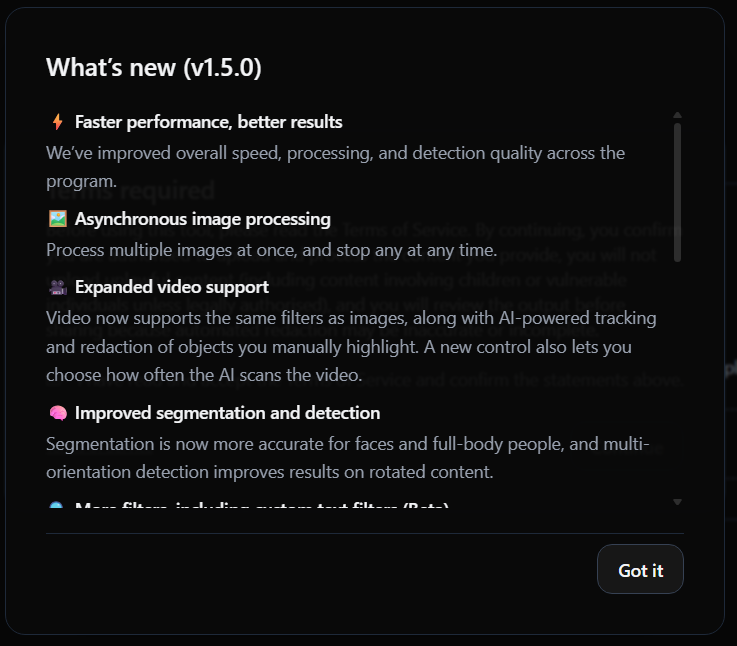
\includegraphics[width=\textwidth, trim=35 35 35 35, clip]{figures/images/chapter-6/PatchNotesExamples.png}
        \caption{Patch notes dialog summarizing user-visible system changes.}
        \label{fig:patch_notes}
    \end{subfigure}

    \caption{Supporting interface dialog for responsible use and system communication.}
    \label{fig:user_guidance_dialogs}
\end{figure}